\chapter{Data and Methodology}
\label{ch:methodology}

This chapter sets out how the question posed in Chapter~\ref{ch:introduction} was turned into something a
dataset can answer. It begins with the research design, the terms that design depends on, and the rule by
which a predictor counts as validated. It then describes the data and the two splits, how the tracker's
performance is measured, and how the label-free features are computed against a frozen reference. The
remaining sections cover the statistical model and the tests applied to it, the replication on a second
dataset and a second tracker, and the constraints that make the work reproducible.

\section{Research design and evaluation criteria}
\label{sec:meth-design}
This is a predictive-modelling study. On one side is a set of predictors $X$: four distances,
each measuring how far a target species or place sits from a frozen reference, none of them requiring the
tracker to be run or the target to be labelled. On the other is a target $Y$: the tracker's per-cell detection
and association scores. The question is whether $X$ predicts $Y$, and which parts of it do the work, asked
separately for the two halves of the task. Nothing here attempts to make the tracker score higher --- it is the
fixed object of study. Three things need pinning down first: what running it zero-shot means, what the two
scores are, and what would count as having predicted them.

\subsection{What ``zero-shot'' means here}
\label{sec:meth-zeroshot}
A model is run zero-shot on a category when it is asked to find that category without having been trained on
labelled examples of it, and without any change to its weights at the time of asking. The only thing telling it
what to look for is the prompt. A conventional detector, by contrast, is trained on a fixed list and can be
asked about nothing else; a fine-tuned model has had its weights updated on target-domain data; a few-shot
model is handed a small number of labelled examples. A zero-shot model gets the word \texttt{"impala"} and
nothing more.

Three commitments follow and hold throughout. The tracker is the public released checkpoint, and its weights
are never updated --- not fine-tuned, not adapted, not calibrated on any part of this data. The only input
identifying the target is the text prompt. And no labelled example of the target species ever reaches the
tracker: the ground-truth masks are read afterwards, to score what it produced and to crop images when building
the distance features (Section~\ref{sec:meth-features}), never to tell it what to look for. The only thing
fitted anywhere in this study is the small regression mapping distances onto scores. Note that zero-shot is
meant relative to the dataset and to the reference frozen inside it, not as a claim about SAM\,3's undisclosed
pretraining corpus --- a scope limit taken up in Section~\ref{sec:limitations}.

\subsection{What is being predicted: finding and following}
\label{sec:meth-targets}
The evaluator compares what the tracker produced against what a human annotated. Both sides consist of
masklets, a masklet being one object's mask followed through the clip frame by frame, and a predicted mask
counts as matching an annotated one when their intersection over union reaches a threshold $\alpha$. Given that
matching, \texttt{pDetA} (detection accuracy) asks whether the right animals were found, rewarding annotated
animals that were located and penalising both animals missed and masks invented where no animal was.
\texttt{pAssA} (association accuracy) asks whether identities were kept, measuring across the matched
detections how consistently one predicted identity corresponds to one annotated identity over time; it falls
when one animal's track is split among several predicted identities, when two identities are swapped, and when
two animals are merged into a single track.

Both lie in $[0,1]$, higher is better, and both are averaged over $\alpha\in\{0.05,\dots,0.95\}$, so neither
depends on one arbitrary choice of how much overlap is close enough (Equation~\ref{eq:phota}). The mask-based
variants are used throughout, SA-FARI being mask-annotated, and neither metric is reimplemented: the official
\texttt{VEval} evaluator is run as supplied and its output read.

The two are not symmetric, and the asymmetry matters. Association is conditional on detection, since an
identity can only be assessed for an animal that was found in the first place. A second consequence is worth
flagging at the outset. Where a clip holds a single animal there is only one identity to keep, so
\texttt{pAssA} is then largely determined by \texttt{pDetA} and carries little variance of its own. How often
that happens is a property of the data rather than of the design, and Chapter~\ref{ch:discussion} reports it;
where it dominates, association is reported as the weak target it is rather than as an independently powered
test. The external replication of Section~\ref{sec:meth-replication} was chosen partly because it does not have
this problem.

\subsection{Definition of success and the decision rule}
\label{sec:meth-success}
The intended deliverable is a validated, out-of-sample predictor of \texttt{pDetA}/\texttt{pAssA} from
label-free distances, with confidence intervals that respect the group structure
(Section~\ref{sec:meth-inference}). A distance is taken to predict transfer only if it clears both bars:
\begin{enumerate}[label=(\roman*),leftmargin=2.4em]
  \item its coefficient's group-cluster-bootstrap 95\% confidence interval (CI) excludes zero; and
  \item the grouped cross-validated model beats a mean-predictor baseline by a margin that is significant under
    a paired group-bootstrap.
\end{enumerate}
The bars are not redundant. Criterion~(i) says a relationship is visible in the data the model was fitted on;
it does not say that relationship holds for a species or place never seen, which is the entire practical claim.
Criterion~(ii) is that test, and its baseline is deliberately humble --- predicting each held-out cell with the
training mean, which is what a practitioner with no predictor would effectively assume. A feature clearing (i)
but not (ii) has been fitted, not validated.

H1 (detection $\leftarrow$ species novelty) and H2 (association $\leftarrow$ environment difficulty) are
supported only when their respective distances meet this bar on the split that isolates them. If neither does
under tests built deliberately to be powerful, the conclusion is H0 --- distance explains little variance ---
which is a substantive result rather than a failure to find one, and motivates the representational-probing
direction of Chapter~\ref{ch:discussion}.


\section{Data, splits, and the analysis unit}
\label{sec:meth-data}
SA-FARI~\cite{safari} is the primary dataset, and everything in this section describes it. The independent
replication runs on a second dataset, BURST, which Section~\ref{sec:meth-replication} covers separately.

Each test is a probe: one video paired with one text prompt. The prompt names a species, which resolves its
taxonomy, and the video supplies the location and the timestamp. Probes are then aggregated into cells, a cell
being one (species, location, time) group. Each cell carries support counts ($n_\text{frames}$,
$n_\text{masklets}$, $n_\text{videos}$), used for weighting and as covariates. The cell is the unit of
analysis throughout: it is what carries a score, and what the regression is fitted on.

Hard negatives --- prompts naming a species that is absent --- are kept, because they carry the false-positive
side of detection. There is one exception. The large pooled inference pass uses a stratified per-species cap to
remain feasible, and under that cap hard negatives are set aside from inference and analysed separately
instead (Section~\ref{sec:meth-fp}).

\paragraph{Two complementary splits.}
SA-FARI's shipped split separates locations but not species (Section~\ref{sec:bg-safari}). Species-distance is
therefore $\approx\!0$ for nearly every cell, so that split cannot test species novelty on its own. Because the
tracker is frozen (Section~\ref{sec:meth-zeroshot}), the shipped split plays no training role and serves only
to define our reference distribution, which leaves us free to repartition the same videos. Inference is run
once --- scoring is per-video and split-agnostic --- and two splits are overlaid on the result:
\begin{description}[leftmargin=1.6em,style=nextline]
  \item[Split A --- species hold-out (primary).] Species from both official splits are pooled and held out one
    at a time, so a held-out species' distance is measured to the nearest remaining species. Species-distance
    varies while the environment stays familiar, which isolates H1.
  \item[Split B --- location hold-out (secondary).] The official split, whose unseen locations isolate H2, and
    whose comparability with the published benchmark carries the initial score-sanity check.
\end{description}
Split A is a constructed hold-out rather than a shipped one. That is legitimate precisely because the model is
frozen, and it is reported as constructed throughout.

Split B yields $1{,}447$ scored cells, spanning $113$ taxonomy-bearing categories and $92$ unseen test
locations. Of those cells $346$ are positive, meaning the queried species is present so that \texttt{pDetA} and
\texttt{pAssA} are defined; the remaining $1{,}101$ are hard negatives, drawn from $1{,}486$ hard-negative
probes. Split A pools the species present in both official splits into $1{,}025$ scored cells.

\section{Measuring transfer}
\label{sec:meth-measure}
Figure~\ref{fig:pipeline} sets out the pipeline as a whole. This section describes its upper path: how the
frozen tracker is run and scored into the target $Y$. Sections~\ref{sec:meth-features}
and~\ref{sec:meth-model} describe the lower path and the modelling.

\begin{figure}[htbp]
\centering
\begin{tikzpicture}[>=Latex, node distance=0.9cm, every node/.style={font=\scriptsize},
  b/.style={draw, rounded corners, align=center, inner sep=3pt, minimum height=0.85cm},
  d/.style={b, fill=black!5}, m/.style={b, fill=blue!12},
  f/.style={b, fill=green!16}, g/.style={b, fill=orange!20}]
  % top row: the frozen measurement path X-fixed, producing the target Y
  \node[d, text width=1.8cm] (vid) {tracking videos + ground truth};
  \node[m, text width=2.2cm, right=0.7cm of vid] (sam) {frozen promptable tracker $\to$ official evaluator};
  \node[d, text width=2.1cm, right=0.7cm of sam] (y) {per-cell \texttt{pDetA} / \texttt{pAssA} ($Y$)};
  % bottom row: the label-free predictor path
  \node[f, text width=3.6cm, below=1.05cm of sam] (dist)
    {four label-free distances (taxonomic, visual, environment, temporal) vs the \textbf{frozen reference} ($X$)};
  % modelling column on the right
  \node[g, text width=2.3cm, right=1.0cm of y, yshift=-0.9cm] (glm) {support-weighted logit GLM \;($X\!\to\!Y$)};
  \node[g, text width=2.3cm, below=0.55cm of glm] (cv)
    {out-of-sample validation: hold out whole species / locations};
  \draw[->] (vid) -- (sam);   \draw[->] (sam) -- (y);
  \draw[->] (vid.south) |- (dist.west);
  \draw[->] (y.east)    -| ([xshift=-1pt]glm.north);
  \draw[->] (dist.east) -- ([xshift=-10pt]dist.east -| glm.west) |- (glm.west);
  \draw[->] (glm) -- (cv);
\end{tikzpicture}
\caption[The measurement-and-modelling pipeline]{The measurement-and-modelling pipeline, identical for every
dataset and tracker. \emph{Top:} the frozen tracker is scored by the official evaluator into per-cell
detection/association scores (the target $Y$). \emph{Bottom:} four label-free distances are computed against a
frozen reference (the predictors $X$). A support-weighted logit GLM relates $X$ to $Y$, validated out of sample
by holding out whole species and locations. Only the GLM is fitted; the tracker is never trained.}
\label{fig:pipeline}
\end{figure}

The primary case is SAM\,3 on SA-FARI, and the rest of this section gives its concrete choices and numbers.
The replication and the model swap (Sections~\ref{sec:meth-replication}--\ref{sec:meth-swap}) later re-run the
same pipeline on other datasets and trackers.

SAM\,3~\cite{sam3} is run frozen over the probe videos and scored with the official \texttt{VEval} evaluator,
which yields a per-cell \texttt{pDetA}, \texttt{pAssA} and \texttt{pHOTA}~\cite{hota} together with its
support. Species-specific prompts are the primary condition, and a generic ``animal'' prompt is run as a
robustness check. One inference pass over the union of the Split~A and Split~B probes serves both experiments.
Predictions are keyed per (video, species), so that the several prompts issued against a single video cannot
collide, and the harness can resume video by video.

The frame-level scores are aggregated two ways, and the two are kept distinct. The micro score is the
dataset-level \texttt{VEval} figure, reported only to confirm that we reproduce the published SA-FARI operating
point of $\approx\!0.65$ mask-\texttt{pHOTA}. The macro score is the support-weighted mean over positive cells,
and it is the modelling target: the model is fitted cell by cell, so the cell is what must carry a score. Being
a positives-only per-cell average, the macro mean sits lower, at $\approx\!0.53$. Unless a figure is explicitly
identified as the micro score, every measurement number quoted in this dissertation is the macro value.

\paragraph{Validity of the frozen protocol.} Because the tracker is frozen throughout
(Section~\ref{sec:meth-zeroshot}), reusing that single inference pass across both splits is sound rather than a
leak: a cell's score cannot depend on which reference partition is later overlaid to compute its distances.

Freezing also settles the benchmark's status. SA-FARI is a held-out, zero-shot benchmark for the released
SAM\,3. The SAM\,3 report~\cite{sam3} does not list SA-FARI among its training sources, and the SA-FARI
paper~\cite{safari} reports the released checkpoint zero-shot, alongside separately fine-tuned rows whose gain
we deliberately forgo. Non-membership can therefore be verified at the dataset level. It cannot be verified
frame by frame, because SAM\,3's full pretraining corpus is undisclosed. That is why every distance is measured
against the SA-FARI reference rather than against whatever SAM\,3 actually saw, and why the familiarity proxy
of Section~\ref{sec:meth-familiarity} is included as a hedge.

\section{Label-free distance features}
\label{sec:meth-features}
The features defined here fall into three groups. Four are distances, one for each axis along which a target
can be unfamiliar: taxonomic, visual, environment and temporal. These four are the hypothesis variables, with
H1 resting on the first two and H2 on the third. The second group holds a single nuisance covariate, animal
size. The third holds the familiarity proxy.

For each split, the reference (``seen'') species, locations and taxonomy are frozen once, and every distance is
then computed against that reference alone. This is the leakage firewall: no information about a probe can
enter a feature. A unit test verifies it, swapping the reference and checking that the distances move as
expected. We assert the axis that is genuinely disjoint --- location for Split~B, the held-out species for
Split~A --- and report any residual species overlap rather than asserting it away.

Because the distances are computed against that reference, they require no measurement of the tracker's
performance on the target: no \texttt{pDetA}, no \texttt{pAssA}, no annotation of how well SAM\,3 did. That is
the sense in which they are label-free, and it is the sense the research question needs, since it makes them
available before the model is run.

One qualification belongs here rather than in a footnote. As implemented on an annotated benchmark, the visual,
environment and size features read the dataset's ground-truth masks to separate animal from scene. That is a
convenience of working on SA-FARI, not a requirement of the method: in deployment the same species prototype
would be built from the handful of exemplar images a practitioner already has for a named species. It does
bound the claim, and Section~\ref{sec:limitations} returns to it.
\subsection{Taxonomic distance}
This distance measures how far apart two species sit on the tree of life.

Every species carries a seven-level path from kingdom down to species. Write that path $\pi(s)$, and let
$\mathrm{shared}(a,b)$ count the levels on which two paths agree, starting from the top. Two species are then
as far apart as the number of levels they do not share. A cell's distance is the smallest such value over the
reference set $\mathcal{R}$:
\begin{equation}
  \tau(a,b)=L-\mathrm{shared}(a,b)\quad (L=7),
  \qquad
  d_{\mathrm{tax}}(s)=\min_{s'\in\mathcal{R},\;s'\neq s}\tau\big(\pi(s),\pi(s')\big).
  \label{eq:taxdist}
\end{equation}

So a species sharing a genus with its nearest reference neighbour scores $1$, a shared family $2$, and a shared
order $3$. A species sharing no level at all would score $7$. The exclusion $s'\neq s$ is the leave-species-out
rule, which keeps the measure non-trivial for species present on both sides of a split. Species whose taxonomy
is incomplete are left undefined rather than imputed.
\subsection{Visual distance}
This distance measures how different one species looks from another.

Each animal is cropped to its ground-truth mask, with the background zeroed, and embedded with
DINOv2~\cite{dinov2}. A species is then summarised by a single prototype: the mean of its embeddings,
renormalised to unit length. The distance from an embedding $v$ to the nearest prototype other than its own is
one minus the largest cosine similarity,
\begin{equation}
  p_j=\frac{\bar v_j}{\lVert \bar v_j\rVert_2},
  \qquad
  d_{\mathrm{vis}}(v)=1-\max_{j\neq e}\, v^{\!\top}p_j ,
  \label{eq:protodist}
\end{equation}
where $e$ indexes the query's own species, excluded again under the leave-species-out rule. A
CLIP~\cite{clip} encoder replaces DINOv2 as a robustness check. The masks come from the annotations
(Figure~\ref{fig:features}b).
\subsection{Environment distance}
This distance measures how different one scene looks from another.

The animal is erased from the frame, its pixels replaced by the mean colour of what remains, and the result is
embedded exactly as above (Figure~\ref{fig:features}c). Here prototypes are formed per location rather than per
species, and $d_{\mathrm{env}}$ is Equation~\ref{eq:protodist} applied to the nearest other location.

Three interpretable covariates come from the same frames. Infrared footage is greyscale, so a pixel's spread
across colour channels, $\max_c f_c-\min_c f_c$, collapses towards zero; a frame counts as achromatic when that
spread averages below $12$. The low-light fraction is the share of a location's frames that are achromatic, and
the night/IR flag is that fraction exceeding one half. Clutter is the mean variance of a Laplacian over the
greyscale background, which measures local edge and texture density rather than colour.

\begin{figure}[htbp]
\centering
\begin{minipage}[b]{0.32\textwidth}\centering
  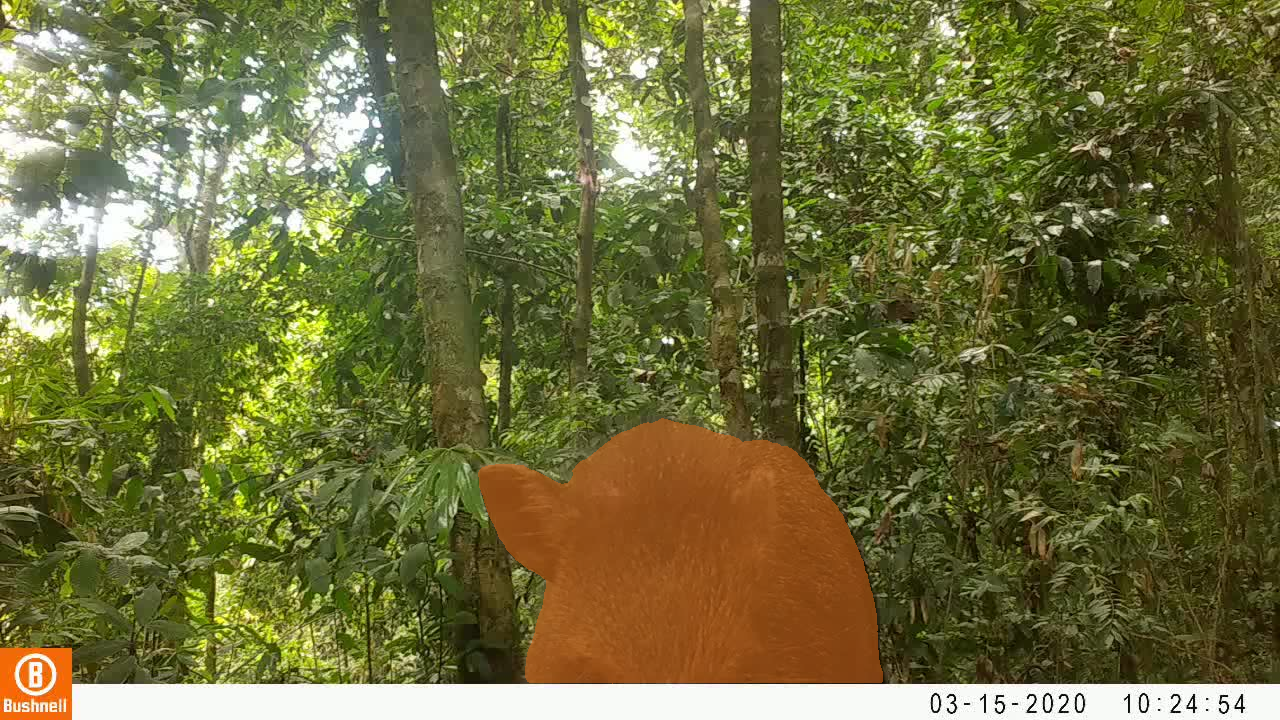
\includegraphics[width=\linewidth]{figures/feat_overlay.png}\\[2pt]{\footnotesize (a) frame $+$ ground-truth mask}
\end{minipage}\hfill
\begin{minipage}[b]{0.32\textwidth}\centering
  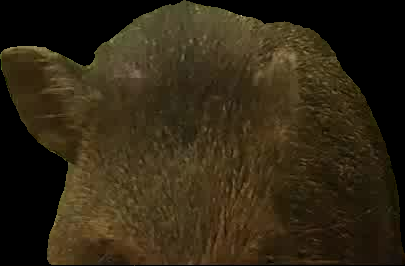
\includegraphics[width=\linewidth]{figures/feat_animal.png}\\[2pt]{\footnotesize (b) visual: mask-cropped animal}
\end{minipage}\hfill
\begin{minipage}[b]{0.32\textwidth}\centering
  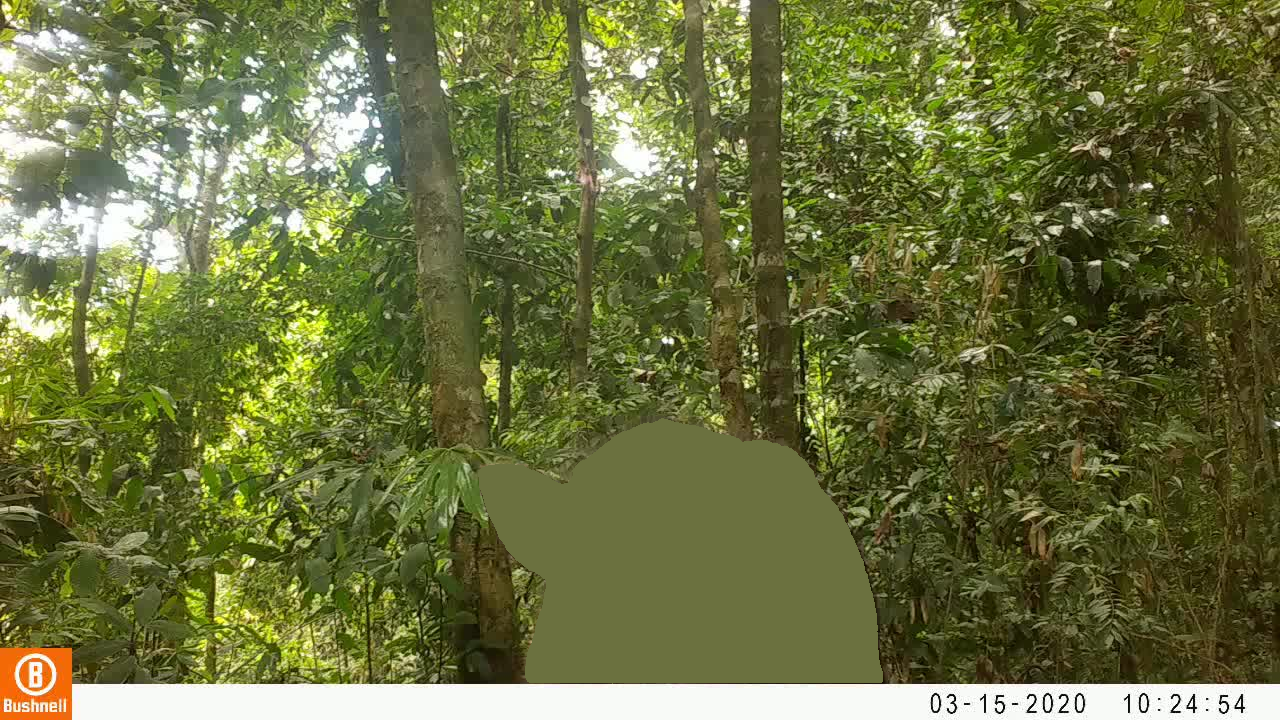
\includegraphics[width=\linewidth]{figures/feat_background.png}\\[2pt]{\footnotesize (c) environment: animal erased}
\end{minipage}
\caption[The image-based distances in action]{The two image-based distances on a camera-trap frame (a collared
peccary). \textbf{(a)} ground-truth mask (orange); \textbf{(b)} the mask-cropped animal the visual
distance fingerprints; \textbf{(c)} the animal mean-inpainted, which the environment distance
fingerprints. None of these features runs SAM\,3.}
\label{fig:features}
\end{figure}

\subsection{Temporal gap}
\label{sec:meth-temporal}
This distance measures how far apart in time two recordings were made.

Years come from the per-video creation-datetime metadata. For a cell recorded in year $y$, the gap is the
smallest absolute difference to any reference year in $\mathcal{Y}$:
\begin{equation}
  d_{\mathrm{temp}}=\min_{r\in\mathcal{Y}}\,|y-r| .
  \label{eq:tempgap}
\end{equation}

The feature depends on timestamps being both present and varied across cells. How far the available metadata
actually supports it is reported in Chapter~\ref{ch:results}.
\subsection{Animal size (confound control)}
This covariate measures how large the animal appears in frame.

Let $a$ be a species' mean ground-truth mask area in pixels, averaged over sampled masklets. The covariate is
$\ln(1+a)$. Larger animals are easier to segment, so this is what separates genuine visual novelty from mere
conspicuousness. Section~\ref{sec:meth-model} describes how it is used to test whether an apparent novelty
effect is really a size effect.
\subsection{SAM\,3 familiarity proxy}
\label{sec:meth-familiarity}
This feature measures how familiar a species looks to SAM\,3 itself.

Every distance above is measured against the SA-FARI reference rather than against what SAM\,3 actually saw
(Section~\ref{sec:meth-measure}). The proxy hedges that gap by reading familiarity from the model. The same
mask-cropped animals used for the visual distance are pushed through SAM\,3's image encoder, and the
patch-token features are mean-pooled into a $1024$-dimensional vector. Each species is then scored three ways:
by silhouette, comparing own-cluster compactness against the nearest other species; by nearest prototype, which
is Equation~\ref{eq:protodist} recomputed with SAM\,3's encoder in place of DINOv2; and by Mahalanobis
typicality against the reference feature Gaussian.

The proxy stays before-running and label-free. It is a property of the images, not a function of SAM\,3's
tracking output, so it is not circular. Each of the three metrics is validated at the same leave-species-out
bar, Bonferroni-corrected across them, and size-controlled. The decisive question is whether any of them adds
out-of-sample gain over the visual distance and size together (Section~\ref{sec:familiarity}).

\section{Statistical modelling and hypothesis testing}
\label{sec:meth-model}
Section~\ref{sec:meth-measure} produced the target $Y$, and Section~\ref{sec:meth-features} the predictors $X$.
This section relates the two, and puts the decision rule of Section~\ref{sec:meth-success} into practice.

Its order follows that rule. The first subsection fits the model, the second derives the confidence intervals
that criterion~(i) tests, and the third the out-of-sample comparison that criterion~(ii) tests. The fourth
divides explained variance between predictors that overlap. The fifth and sixth put two further questions that
the four distances do not reach: whether intrinsic difficulty predicts better than novelty, and whether novelty
predicts false alarms rather than misses. The last checks that the outcome does not hinge on any single design
choice.

\subsection{Per-target regression}
\label{sec:meth-per-target}
Detection and association are modelled separately, because their decomposition is the intellectual core of the
project. Section~\ref{sec:meth-targets} gives the qualification. Association may carry little variance
independent of detection, in which case it is reported as the weaker target rather than as an independently
powered test.

Each target is bounded in $[0,1]$. Each is therefore modelled with a support-weighted logit-link, or
fractional-logit, regression:
\begin{equation}
  \operatorname{logit}\mathbb{E}[y]=x^{\!\top}\beta,
  \qquad\text{fit with variance weights } w=n_{\mathrm{frames}},
  \label{eq:glm}
\end{equation}
where $y$ is the cell's score and $x$ the standardised design. That design carries the four distances, the
scene covariates, and a $\log(n_\text{frames})$ term. The last of these is what keeps ``rare'' from being
mistaken for ``far''.

\subsection{Group-aware confidence intervals}
\label{sec:meth-inference}
A naive model interval would be far too narrow here, for two reasons. Support-weighting by frame count inflates
the effective sample size. And a distance is constant within a species or a location, so hundreds of cells
represent only tens of independent groups, which is pseudo-replication. We therefore resample whole species and
whole locations, refit on each resample, and take percentile intervals. Every coefficient interval reported in
this dissertation is that group-cluster-bootstrap interval.

\subsection{Out-of-sample validation and the significance test}
\label{sec:meth-cv}
Validation holds out whole groups: leave-species-out on Split~A, leave-location-out on Split~B. The model is
fitted without a group, then predicts it. Criterion~(ii) compares the resulting error against the
mean-predictor baseline, and a paired group-bootstrap resampling whole held-out groups tests that comparison.
It returns both a confidence interval and a one-sided $p$-value on the gain.

\paragraph{Distinguishing absence of signal from absence of power.}
A null is only informative if the test could have detected an effect had one been present, so the design
carries a positive control. The animal-size covariate is put through the identical procedure --- the same
clustered interval, the same whole-group hold-out --- and the estimation and cross-validation machinery is
unit-tested to recover planted effects on synthetic data. If the procedure clears the bar for size while
staying flat for the distances, a flat result is evidence of absence of signal rather than absence of power.
Chapter~\ref{ch:results} reports whether it does.

\subsection{Variance attribution and confound control}
\label{sec:meth-variance}
Four univariate fits would not show how much each factor explains, because the distances overlap one another.
Variance is therefore attributed by dominance analysis, which divides shared explanatory power between
correlated predictors, with a VIF check for collinearity. Raw correlations are reported alongside as a
model-free cross-check. Where a distance does reach significance, the model is refitted with the animal-size
covariate, to test whether the effect is size rather than novelty.

\subsection{The intrinsic-difficulty pivot and the nested decomposition}
The novelty distances are not the only label-free properties available. A complementary question, taken up
after the novelty tests were complete, is whether transfer is governed by the intrinsic difficulty of the
target imagery rather than by its novelty. The scene properties already measured for the environment axis ---
the low-light fraction, the clutter score and the night/IR flag --- are promoted from nuisance covariates to
predictors of interest, and tested against the same out-of-sample bar.

Difficulty and size are easily confused, so they are separated by a nested sequence of models: support only,
size only, difficulty without size, and difficulty plus size. Comparing their out-of-sample gains exposes any
apparent difficulty effect that is really size (Table~\ref{tab:difficulty}). Each scene property's cell-level
correlation is also reported beside its location-level value, because aggregating inflates correlations. That
is the ecological-correlation fallacy.

\subsection{Detection precision: false positives on hard negatives}
\label{sec:meth-fp}
The \texttt{pDetA} model conditions on the animal being present, so it measures recall given presence rather
than hallucination. Hard negatives supply the other side. There the queried species is absent, so a correct run
returns no masklet at all.

The predictions are read directly, and any returned masklet scoring above a threshold is flagged as a false
positive. Each species' taxonomic and visual distance is attached, and the test asks whether the hallucination
rate rises with novelty. It is run at the species level rather than the cell level, to avoid pseudo-replication.

\subsection{Design-robustness checks}
\label{sec:meth-robustness}
To test whether the outcome depends on any single design choice, the whole hold-out procedure is re-run with
one component of the pipeline swapped at a time. The visual encoder changes from DINOv2 to CLIP. The crop
changes from the mask-cropped animal to a whole-frame box that keeps the background. The prompt changes from
species-specific to a generic ``animal''. And the visual-distance functional changes from a nearest-prototype
cosine to a distributional Fr\'echet or MMD distance between the target and reference embedding sets, after
AutoEval~\cite{autoeval}. Each variant is fitted and validated at the identical whole-group bar, with
significance judged after a Bonferroni correction over the variant family (Table~\ref{tab:robustness}).

\section{Independent replication on an external dataset}
\label{sec:meth-replication}
Every SA-FARI result reuses one frozen inference pass on one dataset. The two splits are therefore
near-orthogonal, but not statistically independent. To test whether the outcome is a property of the transfer
problem rather than of SA-FARI, the whole pipeline is re-run on a second dataset. Nothing changes but the data:
the same frozen SAM\,3, the same official scorer, the same distances, and the same leave-species-out
cross-validation and paired group bootstrap.

This is cheap because the pipeline is bound to an annotation schema rather than to a loader. An offline adapter
converts the new dataset into the SA-Co JSON that the loader and evaluator already read, so nothing downstream
changes.

\paragraph{BURST.} The replication runs on the animal subset of the BURST validation split
(Section~\ref{sec:bg-burst}): $41$ species across $132$ video\,$\times$\,class cells, scored by mask-HOTA on
the native masks. Animal categories are selected by a WordNet filter~\cite{wordnet}, taking the hyponyms of
\texttt{animal.n.01}, and mapped to the seven-level taxonomy wherever it resolves. It resolves in full for $25$
of the $41$ species, and the rest are left undefined. BURST supplies neither of the metadata axes SA-FARI does,
so the cell key is the per-video sequence and leave-species-out is the only valid grouping. Both
\texttt{pDetA} and \texttt{pAssA} are tested here, at the same bar as SA-FARI and with the same animal-size
positive control (Section~\ref{sec:meth-cv}).

\subsection{The controlled model swap}
\label{sec:meth-swap}
The replication varies the data and holds the tracker fixed. The swap does the reverse. Everything else stays
constant --- the same cells, the same ground truth, the same four distances, the same GLM under
leave-species-out cross-validation --- and SAM\,3 is replaced by another open-vocabulary, text-promptable
tracker. Only \texttt{pDetA} changes, because the distances are functions of the data and its ground truth
rather than of the tracker. That is what isolates the tracker as the sole varying factor, and it is also why
this is a swap rather than a replication.

Two challengers of deliberately different architecture are used. GLEE~\cite{glee} is a single unified
detect--segment--track model. Florence-2~\cite{florence2} paired with SAM\,2~\cite{sam2} is a caption-style box
generator, carrying no confidence score, followed by a mask-propagating tracker.

Two safeguards keep the swap fair. The first is a measurement gate. A challenger's per-cell \texttt{pDetA} must
show real spread across cells before any regression is fitted on it. A regression on scores floored at zero has
no variance to explain and would report a spurious null, so a challenger scoring $\approx 0$ on a dataset is
dropped there rather than modelled.

The second concerns scoring fairness. Open-vocabulary detectors calibrate their confidence to their own
training domain, so a near-zero score may reflect the evaluator's confidence gate rather than a real detection
failure. Every such score is therefore re-checked under a box-based metric, and again under a threshold-free
average-precision metric with no gate at all. This gate is also what decides which dataset can host a fair
swap, and it is why the swap runs on BURST rather than SA-FARI; Chapter~\ref{ch:results} gives the measurements
behind that choice. Each challenger configuration is fixed in advance from the model's own defaults, run once,
and reported as-is (Section~\ref{sec:model_swap}).

\section{Reproducibility and implementation}
\label{sec:meth-repro}
The constraints that protect validity are stated where they apply: the frozen tracker
(Section~\ref{sec:meth-zeroshot}), the official evaluator (Section~\ref{sec:meth-targets}), the frozen
reference (Section~\ref{sec:meth-features}), and the retained hard negatives (Section~\ref{sec:meth-data}).
What remains is how they are enforced.

Each is a configuration toggle rather than a branch in the code, so an ablation changes a config file and
nothing else. The pipeline is covered by hermetic tests, among them the leakage check of
Section~\ref{sec:meth-features} and the recovery of planted effects on synthetic data. Split definitions,
random seeds and reference sets are all persisted. Every number reported in this dissertation comes from that
pipeline, and both experiments reproduce end to end.

All inference is single-GPU and inference-only, since no weights are ever updated.
